% !TeX spellcheck = en_US

\chapter{Analysis}
This chapter is about identifying the requirements, needed to transform the application into a microservice frontend.\\
The Analysis first determines use-cases for the system based on the stakeholders. A gap-analysis is then performed to compare use-cases of the new system in difference to the old one. The result of this process will be requirements, which are separated into functional and non-functional.


\section{Stakeholders}
Stakeholders are groups of people with an interest in the system. This interest can be from a practical user based standpoint, as well as from a management standpoint.

\subsection{Model Developer}
The Model Developer is a technical user that creates a MARS model in cooperation with a domain expert. His main goal is to make sure the model, he created executes correctly and without errors.

\subsection{Simulation Creator}
The Simulation Creator is a domain expert. He Uses the Model, created by the Model Developer to answer a research question. Model Developers goal is, to start various simulations with a given model to validate or invalidate theories. To do so, he mainly changes the parameters of a given scenario to find out, how different parameters effect the result.

\subsection{Group Administrator}
The Group Admin is a user of the system with a leading roll in his group. He wants to manage people belonging to a particular group and handle group dependent settings. He wants to add users to his group, remove them and handle permissions for data, owned by his group.

\subsection{Administrator}
The Administrator is a global user with far reaching permission inside the system. An admin has to be able to alter any kind of data inside the system.


\section{Use-cases}
The workflow that includes completing all the necessary steps to start a simulation, can be broken down into five parts: \textit{Import Data}, \textit{Check imported Files}, \textit{Create Mapping}, \textit{Start Simulation} and \textit{View Results}. This piece of work does not cover the whole workflow. Instead, it is focused on the first three use-cases.\\
The Use-cases \textit{Manage Groups} and \textit{Manage Users} are for administrative purposes only. They are also not part of this paper.\\
Figure \ref{fig:use-cases} shows an overview of the mentioned use-cases with their stakeholders. Note, that although the Model Developer and the Simulation Creator have a different view of the system, the use-Cases do not differ. This is why they are simply referred as user.
\begin{figure}[H]
	\centering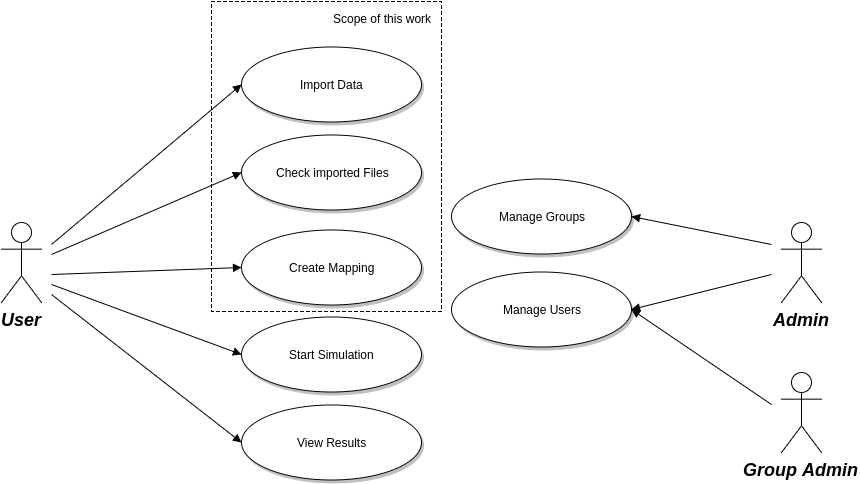
\includegraphics[width=1\textwidth]{res/Use-Cases_reduced}
	\caption{Use-Cases in UML notation}
	\label{fig:use-cases}
\end{figure}

\subsection{Import Files}
\begin{usecase}
	\addtitle{Import I}{Data}
	\addfield{Summary}{Upload local data files to the Websuite, to use them for a simulation.}
	\additemizedfield{Actors}{
		\item User
	}
	\additemizedfield{Preconditions}{
		\item \textit{Import Data} page is open.
	}
	\additemizedfield{Primary Scenario: }{
		\item The user drags one or multiple files onto the upload window, fills the form for every file and starts the import.
	}
	\additemizedfield{Alternative Scenario: }{
		\item The user clicks the upload button, selects files, fills the form for every file and starts the import.
	}
\end{usecase}

\begin{usecase}
	\addtitle{Import II}{Model}
	\addfield{Summary}{Upload local model files to the Websuite, to use them for a mapping.}
	\additemizedfield{Actors}{
		\item User
	}
	\additemizedfield{Preconditions}{
		\item \textit{Import Model} page is open.
	}
	\additemizedfield{Primary Scenario: }{
	\item The user drags one or multiple files onto the upload window, fills the form for every file and starts the import.
	}
	\additemizedfield{Alternative Scenario: }{
		\item The user clicks the upload Window, selects files, fills the form for every file and starts the import.
	}
\end{usecase}

\begin{usecase}
	\addtitle{Import III}{Bulk}
	\addfield{Summary}{Upload multible files to the Websuite, with the same metadata, to save time for files that are handled alike.}
	\additemizedfield{Actors}{
		\item User
	}
	\additemizedfield{Preconditions}{
		\item \textit{Import Data} page is open.
	}
	\additemizedfield{Primary Scenario: }{
		\item The user selects bulk upload, adds the files like for \textit{Import I} and fills one form to handle all the files.
	}
	\additemizedfield{Alternative Scenario: }{
		\item none
	}
\end{usecase}

\subsection{Check imported Files}
\begin{usecase}
	\addtitle{View I}{Search \& filter results}
	\addfield{Summary}{Find specific input data with the help of a search and filter functionality.}
	\additemizedfield{Actors}{
		\item User
	}
	\additemizedfield{Preconditions}{
		\item \textit{Data View} page is open
		\item Files have been imported
	}
	\additemizedfield{Primary Scenario: }{
		\item The user views imported files, filters them by category and sorts them by name.
	}
	\additemizedfield{Alternative Scenario: }{
		\item The user filters by text input and sorts them by category.
	}
\end{usecase}

\begin{usecase}
	\addtitle{View II}{Check processing result}
	\addfield{Summary}{Make sure all the imported files from data- and modelimport were processed correctly.}
	\additemizedfield{Actors}{
		\item User
	}
	\additemizedfield{Preconditions}{
		\item \textit{Data View} page is open
		\item Files have been imported
	}
	\additemizedfield{Primary Scenario: }{
		\item The user checks the status of multible imported files by searching for them.
	}
	\additemizedfield{Alternative Scenario: }{
		\item none
	}
\end{usecase}

\begin{usecase}
	\addtitle{View III}{View metadata}
	\addfield{Summary}{View the metadata of a specific imported file.}
	\additemizedfield{Actors}{
		\item User
	}
	\additemizedfield{Preconditions}{
		\item \textit{Data View} page is open
		\item Files have been imported
	}
	\additemizedfield{Primary Scenario: }{
		\item The user clicks on a specific import entry and views the metadata inside a modal window.
	}
	\additemizedfield{Alternative Scenario: }{
		\item none
	}
\end{usecase}

\subsection{Create Mapping}
\begin{usecase}
	\addtitle{Scenario I}{Create scenario}
	\addfield{Summary}{Create a scenario based on a model.}
	\additemizedfield{Actors}{
		\item User
	}
	\additemizedfield{Preconditions}{
		\item \textit{Create Scenario} page is open
		\item A model has been uploaded.
	}
	\additemizedfield{Primary Scenario: }{
		\item The user clicks the "add Scenario" button. Inside the new modal, he fills the form, selects a model and saves the new scenario.
	}
	\additemizedfield{Alternative Scenario: }{
		\item none
	}
\end{usecase}

\begin{usecase}
	\addtitle{Scenario II}{Create Mapping}
	\addfield{Summary}{Combine the fields from the uploaded model with uploaded data.}
	\additemizedfield{Actors}{
		\item User
	}
	\additemizedfield{Preconditions}{
		\item \textit{Create Mapping} page is open
		\item Data has been imported
		\item Model has been imported
	}
	\additemizedfield{Primary Scenario: }{
		\item The user selects a scenario and starts mapping the required fields to a dataset. He then sets the parameters for the simulation.
	}
	\additemizedfield{Alternative Scenario: }{
		\item none
	}
\end{usecase}


\section{Gap-Analysis}


\section{Requirements}

\subsection{Functional Requirements}

\reqstartF
\item Functional requirement description 1;
\reqendF



\subsection{Non-Functional Requirements}

\reqstartNF
\item Non-functional requirement description 1;
\reqendNF
